%%%%%%%%%%%%%%%%%%%%%%%%%%%%%%%%%%%%%%%%%
% Short Sectioned Assignment LaTeX Template Version 1.0 (5/5/12)
% This template has been downloaded from: http://www.LaTeXTemplates.com
% Original author:  Frits Wenneker (http://www.howtotex.com)
% License: CC BY-NC-SA 3.0 (http://creativecommons.org/licenses/by-nc-sa/3.0/)
%%%%%%%%%%%%%%%%%%%%%%%%%%%%%%%%%%%%%%%%%

%----------------------------------------------------------------------------------------
%	PACKAGES AND OTHER DOCUMENT CONFIGURATIONS
%----------------------------------------------------------------------------------------

\documentclass[paper=a4, fontsize=11pt]{scrartcl} % A4 paper and 11pt font size

% ---- Entrada y salida de texto -----

\usepackage[T1]{fontenc} % Use 8-bit encoding that has 256 glyphs
\usepackage[utf8]{inputenc}
%\usepackage{fourier} % Use the Adobe Utopia font for the document - comment this line to return to the LaTeX default

% ---- Idioma --------

\usepackage[spanish, es-tabla]{babel} % Selecciona el español para palabras introducidas automáticamente, p.ej. "septiembre" en la fecha y especifica que se use la palabra Tabla en vez de Cuadro

% ---- Otros paquetes ----

\usepackage{url} % ,href} %para incluir URLs e hipervínculos dentro del texto (aunque hay que instalar href)
\usepackage{hyperref}
\hypersetup{
	colorlinks=true,
	linkcolor=black,
	urlcolor=black,
	citecolor=black,
}
\usepackage{amsmath,amsfonts,amsthm} % Math packages
%\usepackage{graphics,graphicx, floatrow} %para incluir imágenes y notas en las imágenes
\usepackage{graphics,graphicx, float} %para incluir imágenes y colocarlas

% Para hacer tablas comlejas
%\usepackage{multirow}
%\usepackage{threeparttable}

%\usepackage{sectsty} % Allows customizing section commands
%\allsectionsfont{\centering \normalfont\scshape} % Make all sections centered, the default font and small caps

\usepackage{fancyhdr} % Custom headers and footers
\pagestyle{fancyplain} % Makes all pages in the document conform to the custom headers and footers
\fancyhead{} % No page header - if you want one, create it in the same way as the footers below
\fancyfoot[L]{} % Empty left footer
\fancyfoot[C]{} % Empty center footer
\fancyfoot[R]{\thepage} % Page numbering for right footer
\renewcommand{\headrulewidth}{0pt} % Remove header underlines
\renewcommand{\footrulewidth}{0pt} % Remove footer underlines
\setlength{\headheight}{13.6pt} % Customize the height of the header

\numberwithin{equation}{section} % Number equations within sections (i.e. 1.1, 1.2, 2.1, 2.2 instead of 1, 2, 3, 4)
\numberwithin{figure}{section} % Number figures within sections (i.e. 1.1, 1.2, 2.1, 2.2 instead of 1, 2, 3, 4)
\numberwithin{table}{section} % Number tables within sections (i.e. 1.1, 1.2, 2.1, 2.2 instead of 1, 2, 3, 4)

\setlength\parindent{0pt} % Removes all indentation from paragraphs - comment this line for an assignment with lots of text

\newcommand{\horrule}[1]{\rule{\linewidth}{#1}} % Create horizontal rule command with 1 argument of height
\usepackage{booktabs}

\usepackage{listings}
\lstdefinelanguage
[x64]{Assembler}     % add a "x64" dialect of Assembler
[x86masm]{Assembler} % based on the "x86masm" dialect
{morekeywords={CDQE,CQO,CMPSQ,CMPXCHG16B,JRCXZ,LODSQ,MOVSXD, %
		POPFQ,PUSHFQ,SCASQ,STOSQ,IRETQ,RDTSCP,SWAPGS, %
		rax,rdx,rcx,rbx,rsi,rdi,rsp,rbp, %
		r8,r8d,r8w,r8b,r9,r9d,r9w,r9b, %
		r10,r10d,r10w,r10b,r11,r11d,r11w,r11b, %
		r12,r12d,r12w,r12b,r13,r13d,r13w,r13b, %
		r14,r14d,r14w,r14b,r15,r15d,r15w,r15b}} % etc.
\usepackage{color}
\usepackage{xcolor}
\lstdefinestyle{customc}{
	belowcaptionskip=1\baselineskip,
	breaklines=true,
	frame=L,
	xleftmargin=\parindent,
	language=C,
	showstringspaces=false,
	basicstyle=\footnotesize\ttfamily,
	keywordstyle=\bfseries\color{green!40!black},
	commentstyle=\itshape\color{purple!40!black},
	identifierstyle=\color{blue},
	stringstyle=\color{orange},
}

\lstset{escapechar=@,style=customc}
\usepackage{url}

\title{	
	\normalfont \normalsize
	\begin{figure}[htb]
		\centering
		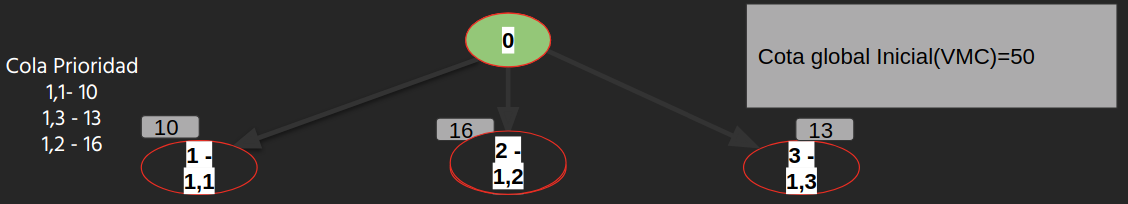
\includegraphics[width=0.3\textwidth]{./imagenes/1}
	\end{figure}
	\textsc{\textbf{Algoritmica} \\ Grado en Ingeniería Informática \\ 
	Curso 2018-2019} \\ [25pt] 
	\begin{figure}[htb]
		\centering
		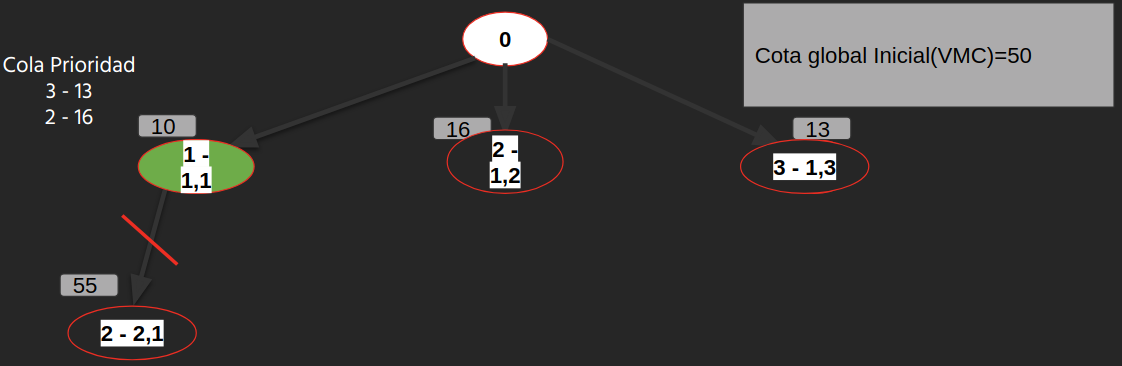
\includegraphics[width=0.15\textwidth]{./imagenes/2}
	\end{figure}
	\horrule{0.5pt} \\[0.4cm]
	\huge Ejercicio Propuesto. \\
	\huge Cambio de monedas
	\\ 
	\horrule{2pt} \\[0.5cm] 
}
\author{Félix Ramírez García  \\
\href{mailto:felixramirezgarcia@correo.ugr.es}{felixramirezgarcia@correo.ugr.es}}
\date{\normalsize\today} 

%----------------------------------------------------------------------------------------
% DOCUMENTO
%----------------------------------------------------------------------------------------

\begin{document}
	
	\maketitle % Muestra el Título
	
	\newpage %inserta un salto de página
	
	\tableofcontents % para generar el índice de contenidos
	
	\listoffigures % para generar índice de imágenes.
	
	\listoftables % para generar índice de tablas.
	
	\newpage
	
	%-----------------------------------------------------------------------
	%							Introduccion
	%----------------------------------------------------------------------	
	\section[Introducción]{Introducción}
	
	El objetivo de esta practica es estudiar cómo habría que modificar el planteamiento del problema de dar cambio resuelto por programación dinámica para el caso en que el número de monedas de cada tipo no sea ilimitado. Para ello vamos a empezar explicando como funciona el algoritmo con numero de monedas ilimitado y luego concluiremos con las modificaciones que realizaremos sobre esta versión para que de solución a un problema con un numero limitado de monedas. 
	

	%-----------------------------------------------------------------------
	%							Solucion con monedas ilimitadas
	%----------------------------------------------------------------------	
	\section[Solución con monedas ilimitadas]{Solución con monedas ilimitadas}
	
	Este algoritmo de programación dinámica sirve para calcular el número  de monedas a retornar de una determinada suma y la cantidad de cada tipo de moneda. Para ello pasaremos como parámetro la cantidad a retornar y un vector con el valor de  los diferentes tipos de monedas. Finalmente el algoritmo retorna un vector con la cantidad de cada tipo de monedas a devolver. \\
	
	En primer lugar debemos pensar como plantear el problema de forma incremental. Consideramos el tipo de moneda de mayor valor, XN. Si XN > C entonces la descartamos y pasamos a considerar monedas de menor valor. Si XN < C tenemos dos opciones: \\
	
	-tomar una moneda de tipo XN, y completar la cantidad restante C – XN con otras monedas\\
	-no tomar ninguna moneda de tipo XN Y completar la cantidad C con monedas de menor valor.\\
	
	 De las dos opciones nos quedamos con la que requiera un número menor de monedas. El problema lo podemos expresar de la siguiente forma cuando consideramos N tipos de monedas: \\
	 
	\lstset{language=C}
	\begin{lstlisting}[frame=single]
Cambio(N,C) = cambio(N-1,C) si XN > C
	      MIN(cambio(N-1),cambio(N,C-XN)+1) si XN <=C
	\end{lstlisting} 
	 	
	.\\
	 Podemos razonar análogamente para monedas de valores k menores que N y para cantidades C’ menores que C. \\
	 
	 \lstset{language=C}
	\begin{lstlisting}[frame=single]
Cambio(K,C') = Cambio(K-1,C') si xk > C'
               MIN(cambio(K-1,C'),cambio(N,C'-Xk)+1) si k >= C'
	\end{lstlisting} 
	
	.\\
	
	Llegamos a los casos base de la recurrencia cuando completamos la cantidad C (1), o cuando ya no quedan más tipos de monedas por considerar, pero aún no se ha completado la cantidad C (2).\\
	
	(1)	cambio(k,0) = 0 si 0<= k <=n  \\
	(1)	cambio(0,C’) = infinito si 0< C’ <= C \\
	
	
	Podemos construir una tabla para almacenar los resultados parciales que tenga una fila para cada tipo de moneda y una columna para cada cantidad posible entre 1 y C. Cada posición t[i,j] será el número mínimo de monedas necesario para dar una cantidad j con 0 <= j <= c utilizando sólo monedas de los tipos entre 1 e i, con 0 <=i<=n .\\
	
	La solución al problema será por tanto el contenido de la casilla t[N,C].\\
	
	Para construir la tabla empezamos rellenando los casos base t[i ,0] = 0, para todo i con 0 <= i  <=  n . A continuación podemos rellenar la tabla bien por filas de izquierda a derecha, o bien por columnas de arriba a abajo. \\
	
	Siguiendo el método de la programación dinámica, se rellena una tabla con las filas correspondientes a cada valor para las monedas y las columnas con valores desde el 1 hasta el N (12 en este caso) . Cada posición (i, j) de la tabla nos indica el número mínimo de monedas requeridas para devolver la cantidad j con monedas con valor menor o igual al de i. La siguiente imagen muestra un ejemplo en que se tiene que devolver cambio de 12 y tenemos monedas de 1 , 6 y 10. Pudiendo pagar con 12 monedas de 1 , 2 monedas de 6 o una e 10 y dos de uno, quedándonos con la mejor opción que seria la que menos monedas tuviera, dos de 6 en este caso .   \\
	
	
	\begin{figure}[htb]
		\centering
		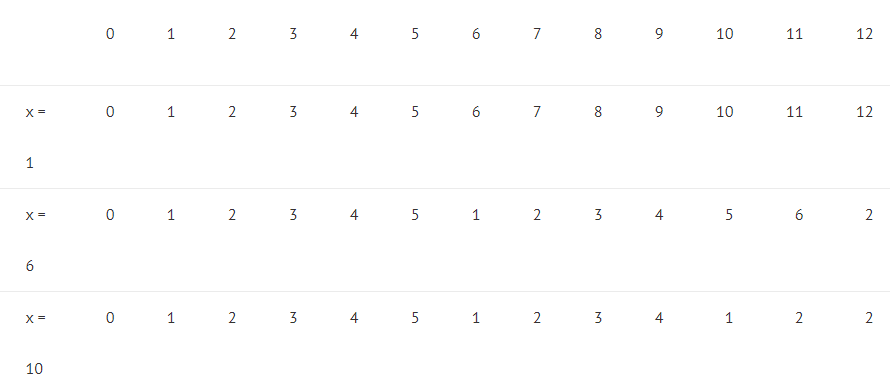
\includegraphics[width=1.0\textwidth]{./imagenes/3}
		\caption{Tabla ejemplo a devolver 12 con monedas de 1,6,10.} \label{fig:1}
	\end{figure}
	
	Una descripción del algoritmo seria: \\
	
		\lstset{language=C}
	\begin{lstlisting}[frame=single]
-Para cada casilla de la tabla hacer:
	-Si el valor de la moneda actual es mayor que la cantidad, se paga con el resto de monedas, es decir, se toma el resultado de la casilla superior.

	-Si el valor de la moneda actual es menor o igual que la cantidad, se toma el minimo entre:
		-Pagar con el resto de monedas, tomando el resultado de la casilla superior.
		-Pagar con una moneda del tipo actual y el resto con el resultado que se hubiera obtenido al pagar la cantidad actual a la que se le ha restado el valor de la moneda actual.
	-Tomar como resultado el valor de la ultima celda.
	\end{lstlisting} 
	
	Para saber que tipo de monedas hay que devolver partimos de la casilla final. Para cada casilla t[i,j] el algoritmo va comprobando si su valor ha variado respecto a la casilla de la fila superior. \\
	
	Si no ha variado podemos deducir que no se ha empleado ninguna moneda del tipo de la fila i, y pasamos a comprobar la casilla superior t[i-l j].  \\
	Si ha variado, anotamos que se ha utilizado una moneda de ese tipo Xi y nos movemos a la casilla t[i, j-moneda[i]], para ver qué monedas se han utilizado para dar la cantidad restante.\\
	
	Siguiendo esta estrategia terminaremos alcanzando la casilla t[0,0] en la que ya no queda ninguna cantidad pendiente. Esto se hace en el método seleccionMonedas()\\
	 
	Resumiendo ,si tenemos un vector con los tipos de monedas {1,6,10} y queremos saber la cantidad de monedas necesarias para dicho cambio y que tipo de monedas es, el vector que retornara será {0,2,0} es decir 0 monedas de la cantidad 1, 2 monedas de la cantidad 6 y 0 monedas de la cantidad 10. \\
	
	Para estudiar el coste del algoritmo calculamos el tamaño de la tabla que hay que construir: N x (C + 1). Como las operaciones aritméticas involucradas son de coste constante,  el tiempo de ejecución está en O(NC). \\
	
	A continuación se muestra el código de la implementan de este algoritmo en lenguaje Java: \\
	
	\lstset{language=C}
	\begin{lstlisting}[frame=single]
public class Cambio
{
private int[][] matrizCambio;
private int[] vectorMonedas;
private int cantidad;
private int[] vectorSeleccion;

Cambio(int cantidad, int[]  monedas){
	this.cantidad = cantidad;
	this.vectorMonedas = monedas;
	matrizCambio = calcularMonedas(cantidad, monedas);
	vectorSeleccion = seleccionarMonedas(cantidad, monedas, matrizCambio);
}

public int[] getVectorSeleccion(){
	return this.vectorSeleccion;
}

private int[][] calcularMonedas(int cantidad, int[]  monedas){
	int[][] matrizCambio = new int[monedas.length + 1][cantidad + 1];

	for (int i = 0; i < monedas.length; i++) matrizCambio[i][0] = 0;
	
	for (int j = 1; j <= cantidad; j++) matrizCambio[0][j] = 99;
	
	for (int i = 1; i <= monedas.length; i++)
	for (int j = 1; j <= cantidad; j++) {
		if (j < monedas[i - 1])	matrizCambio[i][j] = matrizCambio[i - 1][j];
		else {
			int minimo = 0;
			minimo = min(matrizCambio[i - 1][j] , matrizCambio[i][j- monedas[i - 1]] + 1);
			matrizCambio[i][j] = minimo;
		}
	}

	return matrizCambio;
}

private int[] seleccionarMonedas(int c, int[] monedas, int[][]tabla ){
	int i,j;
	int[] seleccion = new int[monedas.length];
	for(i = 0; i< monedas.length; i++) seleccion[i]=0; 
	i= monedas.length;         
	j= c;         
	while(j>0){
		if(i>1 && tabla[i][j]==tabla[i-1][j]) i--;
		else{
			seleccion[i-1]++;
			j = j - monedas[i-1];
		}
	}
	
	return seleccion;
}

private int min(int a, int b){
	if(a<b)	return a;
	else return b;
}

}
	\end{lstlisting} 
	
	
	Para llamar a la clase con el ejemplo anterior haríamos :\\
	
	Cambio c = new Cambio(12, new int[]{1,6,10}) \\
	
	y con c.getVectorSeleccion(); obtendríamos el vector con las cantidades de cada moneda cuyo indice se corresponde con los tipos de monedas que pasamos al constructor.
	
	
	%-----------------------------------------------------------------------
	%							Solucion con monedas limitadas
	%----------------------------------------------------------------------	
	\section[Solución con monedas limitadas]{Solución con monedas limitadas}
	
	
	Para el caso de que tengamos un numero de monedas limitado tendríamos que agregar otro vector con los mismo elementos que tipos de monedas diferentes tengamos. Para el ejemplo explicado serian 3 elementos. Luego los valores del vector serian la cantidad de monedas de cada tipo . Por ejemplo si tenemos los tipos de monedas [1,6,10] un vector cantidad podría ser [2,4,8]. De forma que cada vez que se entregue una moneda de un determinado tipo restas uno a la cantidad de esa moneda en el vector de cantidades. En el caso de que ya no se tengan monedas para solventar el problema se indicaría un mensaje de error o se lanzaría una excepción. 


	%-----------------------------------------------------------------------
	%							BIBLIOGRAFIA
	%-----------------------------------------------------------------------
	% Referencia a bibliografia			En \cite{Baz}
	% Referencia a figura				La figura (\ref{fig:1})
	% Espacio entre lineas				\vspace{0.06in}
	% Figura con comentario al pie
	%\begin{figure}[htb]
	%	\centering
	%	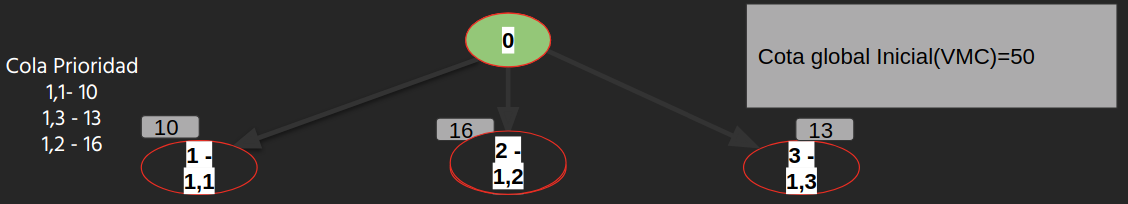
\includegraphics[width=0.4\textwidth]{./imagenes/1}
	%	\caption{Universidad de Granada.} \label{fig:1}
	%\end{figure}
	%\begin{thebibliography}{99}
	%	\bibitem{Baz} 
	%	\textsc{Bazaraa, M.S., J.J. Jarvis}
	%	\textit{Programacuib}.
	%	\newline
	%	\url{https://www.google.es}	
	%\end{thebibliography}

	


\end{document}